\documentclass{article}
\usepackage[a4paper, total={6in, 8in}]{geometry}


% Packages
\usepackage{amsmath}
\usepackage{graphicx}
\usepackage{stmaryrd} 
\usepackage{cite}
\usepackage{listings}
\usepackage{cleveref}
\usepackage{tikz}
\usepackage{subcaption}

\usepackage{amsthm}
\usepackage{amsmath}
\usepackage{amssymb}
% Environnements pour les définitions, théorèmes et propositions
\newtheorem{definition}{Definition}[section]
\newtheorem{theorem}{Theorem}[section]
\newtheorem{proposition}{Proposition}[section]
\newtheorem{lemma}{Lemma}[section]
\newtheorem{problem}{Problem}[section]
\newtheorem*{example}{Example}
\newtheorem{exercise}{Exercise}
\newtheorem{corollary}{Corollary}

% Define the "problem" environment for cleveref
\crefname{problem}{problem}{problems}
\Crefname{problem}{Problem}{Problems}


% Title and Authors
\title{\textbf{Interval Graphs}\\
\large Structure vs Algorithmic Aspects:\\
Which Problems Become Easy and Which Remain Hard?}
\author{Côme Périn}

\begin{document}

\date{December 22, 2024}
\maketitle

\section{Introduction}

\begin{definition}
    \textbf{Intersection Graph} \\
    An Intersection graph $G$ is formed from a family of sets $(S_i)_i$. 
    Each set $S_i$ is represented by a vertex $v_i$ in $G$. 
    Two vertices $v_i$ and $v_j$ are adjacent in $G$ 
    if and only if $S_i \cap S_j \neq \emptyset$ \cite{erdos}. 
\end{definition}

\begin{proposition}
    Every graph is an intersection graph.
\end{proposition}

\begin{proof}
    Let $G$ be a graph. $G$ is an intersection graph with the family of sets 
    $(S_i)_i$ where $S_i$ is the set of neighbors of the vertex $v_i$ in $G$.
\end{proof}

\begin{definition}
    \textbf{Interval Graph} \\ 
    An interval graph is an intersection graph of a 
    set of intervals on the real line $\mathcal{R}$ \cite{golumbic}.

    \begin{figure}[h]
        \centering
        \includegraphics[width=0.5\textwidth]{rsc/interval_graph.png}
        \caption{Some intervals and their corresponding interval graph \cite{wiki_interval}.}
        \label{figure:interval_graph}
    \end{figure}
\end{definition}

\section{Chordality and Perfection}

\begin{definition}
    \textbf{Chord} \\
    A chord of a cycle $C$ is an edge which is not in $C$ but is adjacent to vertices of $C$ \cite{on_chordal}.
\end{definition}

\begin{definition}
    \textbf{Chordal Graph : } \\
    A graph $G$ is chordal if every cycle of length four or
    more in $G$ has a chord in $G$ \cite{on_chordal}.
\end{definition}

\begin{theorem}
    Intervals graphs are chordal graphs.
    \label{theorem:interval_is_chordal}
\end{theorem}

\begin{proof}
    Let $G$ be an interval graph. \\
    Let $C$ be a cycle of $G$ of length $\geq 4$ \emph{without any chords}. \\
    Without loss of generality we can consider that the cycle is of length $4$.

    \bigskip

    \begin{figure}[h]
        \centering
        % Première sous-figure
        \begin{subfigure}[t]{0.45\textwidth}
            \centering
            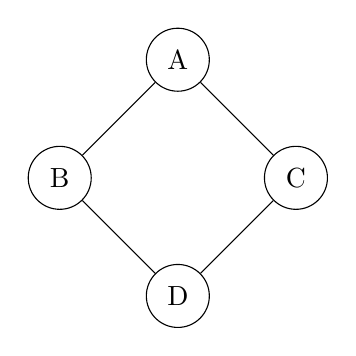
\begin{tikzpicture}[scale=1.5, every node/.style={circle, draw, minimum size=0.8cm, inner sep=0pt}]
                % Les sommets
                \node (A) at (0, 1) {A};
                \node (B) at (-1, 0) {B};
                \node (C) at (1, 0) {C};
                \node (D) at (0, -1) {D};
    
                % Les arêtes
                \draw (A) -- (B);
                \draw (A) -- (C);
                \draw (B) -- (D);
                \draw (C) -- (D);
            \end{tikzpicture}
            \caption{$C_4$.}
            \label{fig:diamond_graph}
        \end{subfigure}
        \hfill
        % Deuxième sous-figure
        \begin{subfigure}[t]{0.45\textwidth}
            \centering
            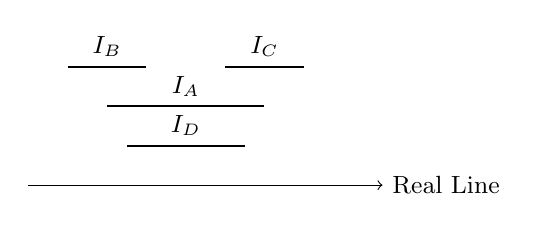
\begin{tikzpicture}[scale=1, every node/.style={font=\small}]
                \def\spacing{0.5}
                \draw[thick] (0, 3*\spacing) -- (1, 3*\spacing) node[midway, above] {$I_B$};
                \draw[thick] (2, 3*\spacing) -- (3, 3*\spacing) node[midway, above] {$I_C$};
                \draw[thick] (0.5, 2*\spacing) -- (2.5, 2*\spacing) node[midway, above] {$I_A$};
                \draw[thick] (0.75, 1*\spacing) -- (2.25, 1*\spacing) node[midway, above] {$I_D$};
            
                \draw[->] (-0.5, 0) -- (4, 0) node[right] {Real Line};
            \end{tikzpicture}
            \caption{Interval representation of $C_4$.}
            \label{fig:interval_representation}
        \end{subfigure}
        \caption{Interval representation of a cycle $C_4$.}
        \label{fig:side_by_side}
    \end{figure}

    According to the definition of a $C_4$ (see \cref{fig:diamond_graph}),
    we must have $I_B \cap I_D \neq \emptyset$ and $I_C \cap I_D \neq \emptyset$. \\
    It is clear that looking at \cref{fig:interval_representation}, this implies
    that $I_A \cap I_D \neq \emptyset$ which is a contradiction. \\

\end{proof}

\begin{definition}
    \textbf{Perfect elimination ordering} \\ 
    A perfect elimination (PEO) of a graph $G$ 
    is an ordering of the vertices of $G$
    such that for each vertex $v$, $v$ and the neighbors of $v$ 
    succeding $v$ in the ordering, form a clique \cite{rose}.
\end{definition}

\begin{example}
    a perfect elimination ordering of the graph featured in \cref{figure:interval_graph} is
    \texttt{GFEDCAB}
\end{example}

\begin{theorem}
    Let $G$ be a graph. The following are equivalent:
    \begin{enumerate}
        \item $G$ is chordal.
        \item $G$ has a perfect elimination ordering.
    \end{enumerate}
    \label{theorem:chordal_is_peo}
\end{theorem}

\begin{proof}
    The proof is given by \cite{rose}.
\end{proof}


\newpage

\begin{proposition}
    \label{proposition:peo_linear}
    A PEO ordering of a graph is computable in linear time \cite{mario}.
\end{proposition}

\begin{proof}
    Several processes can be used to compute a PEO, this proof is given by \cite{mario}
    and uses the following \emph{maximum cardinality search} algorithm. \\

    Let $G$ be a graph with $|V(G)|=n$.

    \begin{lstlisting}[mathescape=true, caption={Maximum Cardinality Search}, label={lst:MCS}, frame=single]
        $W \leftarrow V(G)$
        $\forall v \in W, weight(v) \leftarrow 0$
        for $i$ in $[1, \dots, n ]$ do :
            $u \leftarrow v \in W \text{ where } weight(v) = max\{weight(v') \mid v' \in W\}$
            $v_{n-i+1} \leftarrow u$
            for $i$ in $neighbors(u, W)$ do :
                $weight(w) \leftarrow weight(w)+1$
            $remove(u, W)$
        return $v_1, v_2 \dots v_n$
    \end{lstlisting}
    


\end{proof}

\begin{definition}
    \textbf{Perfect graph} \\
    A graph $G$ is perfect if, for every induced subgraph $H$ of $G$ 
    the chromatic number of $H$ equals the size of the largest clique $\omega(G)$ in $H$ \cite{Chudnovsky2003}.
\end{definition}


\begin{lemma}
    Let $G$ be a chordal graph, then $\mathcal{X}(G)=\omega(G)$.
    \label{lemma:ki_g_eq_omega_g}
\end{lemma}

\begin{proof}
    Let $G$ be a chordal graph.\\
    According to \cref{theorem:chordal_is_peo}, $G$ has a \emph{perfect elimination ordering}
    $(v_i)_{i\in \llbracket 1, V(G) \rrbracket}$. \medskip

    \noindent Let be $\{c_i\}_i = \llbracket 1, \omega(G)\rrbracket$ a set of colors. \\
    Let us use a greedy algorithm to color $G$ :
    
    \begin{lstlisting}[mathescape=true, caption={Greedy algorithm for coloring a chordal graph}, label={lst:greedy_coloring}, frame=single]
        for $k$ in $\lbrack | V(G) |, \; \dots \;, 2\rbrack$ do
            $v_k \leftarrow$ smallest_available_color_among_neighbors_for($v_k,\{c_i\}_i$)
    \end{lstlisting}
    

    \noindent This greedy algorithm gives a correct coloring of $G$ providing that there are enough colors in $\{c_i\}_i$.
    According to the definition of the PEO $v_k$ as at most $\omega(G)-1$ neighbors after itself in the PEO. \\
    \noindent Thus, $\mathcal{X}(G) \leq \omega(G)$ which leads to $\mathcal{X}(G)=\omega(G)$.
\end{proof}


\begin{lemma}
    Let $H$ be a subgraph of $G$. If $G$ is chordal then $H$ is chordal.
    \label{lemma:ind_sub_of_chord_is_chord}
\end{lemma}

\begin{proof}
    Let suppose $G$ is chordal and $H$ is not chordal. \\
    Then there exists a cycle $c$ of length more than $4$ and without chords in $H$. \\
    This cycle also exists in $G$ but it has at least one chord ($G$ being chordal). \\
    So this chord has been removed in $H$, but $H$ is an \textbf{induced subgraph}, so an adjacent vertex to the chord have been removed. \\
    So $c$ is not a cycle in $H$, which is a contradiction.\\
\end{proof}


\newpage

\begin{theorem}
    \label{theorem:interval_is_perfect}
    Interval graphs are perfect graphs
\end{theorem}
    
\begin{proof}
    Let $G$ be an interval graph and $H$ a subgraph of $G$.\\
    According to \cref{theorem:interval_is_chordal}, $G$ is chordal, so, using \cref{lemma:ind_sub_of_chord_is_chord}, $H$ is chordal.\\
    Moreover, using \cref{lemma:ki_g_eq_omega_g}, we have $\mathcal{X}(H)=\omega(H)$. \medskip

    Finally, $G$ is perfect.
\end{proof}

\section{Recognition, Reconstruction and Optimization}

\begin{proposition}
    Given $n\in \mathbb{N}$ intervals $\{I_i\}_{i\in\llbracket 1, n \rrbracket}$ the related interval graph is constructible in $O(n\log(n))$.
\end{proposition}

\begin{proof}
    Each starting or ending point is sorted in an array ($O(n\log{n})$, merge sort for instance) : \\ 
    \textit{e.g.} \lstinline![Start_1, Start_2, End_1, Start_3, End_3, End_2]!.
    While reading this array of event ($O(n)$), an \emph{active set} is updated :

    \begin{itemize}
        \item If an interval starts, it is added to the \emph{active set}.
        A vertex representing the interval is added to the graph and an edge is drawn between 
        this vertex and all other vertices representing intervals of the \emph{active set}.
        \item If an interval ends, it is removed from the \emph{active set}.
    \end{itemize}

    If two interval overlap, it is clear that they will be together in the \emph{active set} at a given moment and thus, 
    they would be adjacent in the graph. This procedure operates $O(n\log(n))$.

    \textbf{NB.} A counting sort might be used ensuring a better complexity of $O(n+k)$ where $k$ is a constant (this is not detailed here).
\end{proof}

\begin{theorem}
    \label{theorem:interval_recognition}
    Interval graphs are recognizable in linear time.
\end{theorem}

\begin{proof}
The proof is given by \cite{booth} and will not be detailed here.
However, the characterization of interval graphs used is the following : \\
A graph $G$ is an interval graph if and only if there exists 
an ordering of the cliques of $G$ such that 
$\forall v\in V(G), \text{ elements of } C(v) \text{ are consecutive in this ordering}$. \\
$C(v)$ denotes the set of cliques containing $v$. \\

\cite{isomorphism} summarizes the idea of the proof by giving the following recognition algorithm : \\

    \begin{lstlisting}[mathescape=true, caption={Interval graph recognition algorithm}, label={lst:interval_recognition}, frame=single]
        if $G$ is not chordal then return False #linear
        $\Pi \leftarrow$ all ordering of the cliques of $G$
        for each $v \in V(G)$ do
            remove from $\Pi$ all ordering where 
            elements of $C(v)$ are not consecutive
        if $\Pi$ is not empty then return True
        return False
    \end{lstlisting}

    The complexity of this algorithm mostly depends on the size of the set $\Pi$.
    Booth and Lueker have introduced \textbf{PQ-trees} to represent the set of all possible 
    orderings of the cliques of a graph and thus operating the algorithm in linear time.
    See \cref{proof:isomorphism} for more details.

\end{proof}

\begin{corollary}
    \label{corollary:interval_reconstruction}
    Given an interval graph $G$, a set of intervals that generates $G$ is constructible in linear time.
\end{corollary}

\begin{corollary}
    \label{corollary:interval_optimization}
    Given an interval graph $G$, it is possible to find an interval reconstruction in linear time (\cref{corollary:interval_reconstruction}) 
    and to operate dynamic programmation on these interval as it can be more efficient than operating on the graph (\emph{e.g.} \texttt{DOMINATION} \cref{proof:domination}).
\end{corollary}

\begin{theorem}
    \label{theorem:exclusion_characterization}
    A graph $G$ is an interval graph if and only if it does not contains a subgraph which is one the graphs $\mathrm{I}, \mathrm{II}, \mathrm{III}_n, \mathrm{IV}_n, \mathrm{V}_n$.
    \begin{figure}[h]
        \centering
        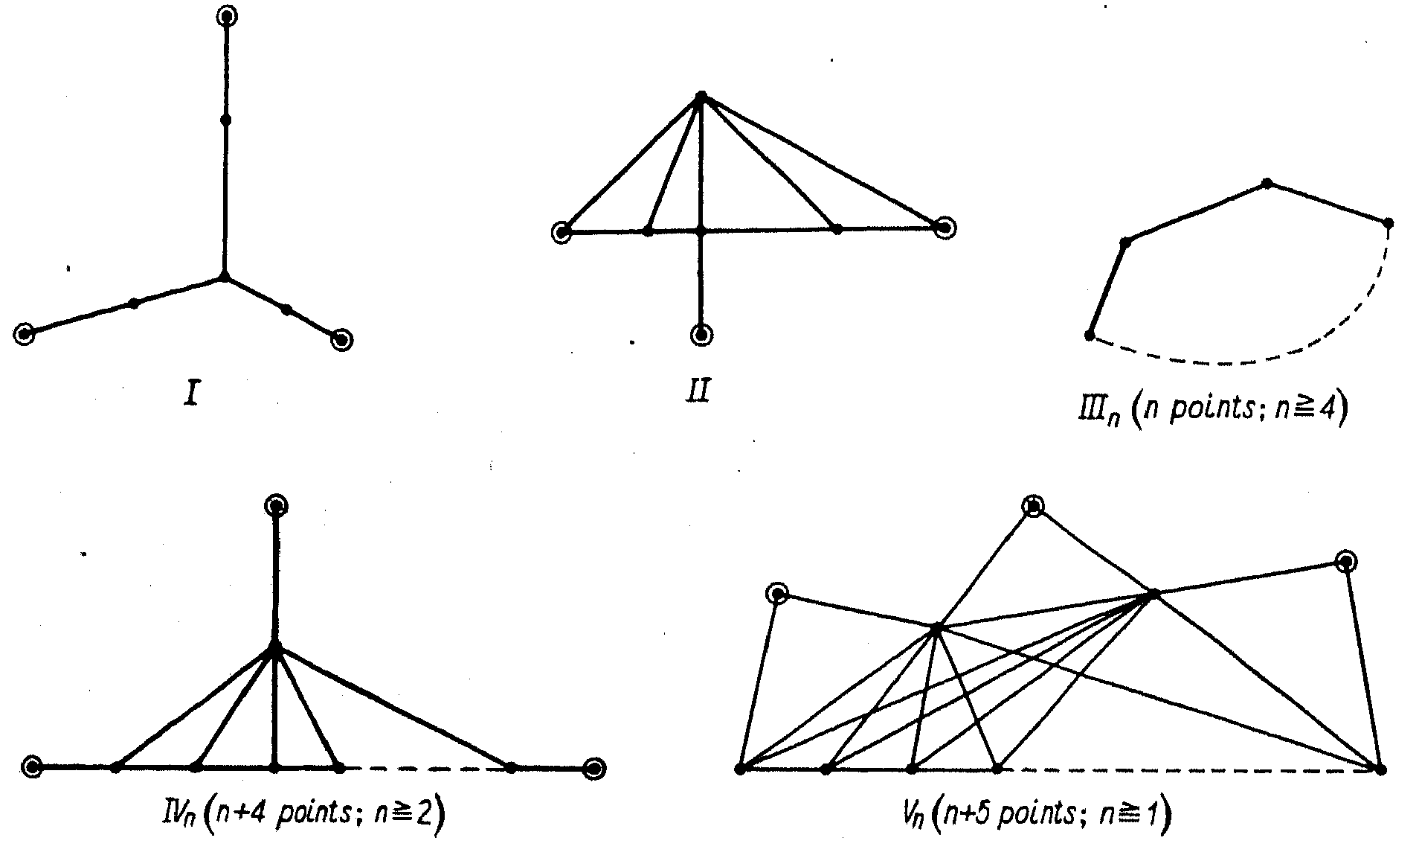
\includegraphics[width=0.9\textwidth]{rsc/forbidden_subgraphs.png}
        \caption{The five forbidden subgraphs \cite{boland}.}
        \label{figure:exclusion_characterization}
    \end{figure}
\end{theorem}

\begin{proof}
    It was one the first characterization of interval graphs, given in 1962 by Lekkerkerker \& Boland \cite{boland}.
\end{proof}

\section{Complexity : What is easier and what remains hard}

Some famous problems are known to be NP-hard for general graphs.
We will study the complexity of some of these problems when restricted to interval graphs.

\subsection{\texttt{CLIQUE}}

This section aims to study the CLIQUE problem on interval graphs.

\begin{problem}
    \label{problem:clique}
    \texttt{CLIQUE}\\
    \texttt{INPUT : } A graph $G$ and a positive integer $k$.\\
    \texttt{OUTPUT : } True if $G$ has a clique of size $k$, False otherwise. 
\end{problem}

\texttt{CLIQUE} is NP-complete for general graphs %\cite{karp}.

\begin{theorem}
    \label{theorem:clique_is_p}
    \texttt{CLIQUE} restricted to interval graphs is linear.
\end{theorem}

\begin{proof}
    Let $G$ be an interval graph.\\
    According to \cref{theorem:interval_is_chordal}, 
    $G$ is chordal, so we can find a PEO of $G$ (\cref{theorem:chordal_is_peo}) 
    in linear time $O(| V(G)|+| E(G)|)$ (\cref{proposition:peo_linear}). \medskip

    Let us consider the following procedure : \\
    For each vertex $v$ in the PEO ($O(| V(G)|)$), compute neighbors of $v$ succeeding $v$ in the PEO ($O(| E(G) |)$ after all calculations). \\
    If $v$ has more than $k-1$ neighbors, return \texttt{True}. \\
    If there is no vertex left to explore, return \texttt{False}. \medskip

    So the complexity of the procedure is $O(|V(G)|+|E(G)|)$. \medskip

    The procedure is correct according to the definition of PEO : 
    if there is a clique in $G$, the clique will appear in the procedure as soon as one of the vertex of the clique is explored.
\end{proof}

\textit{NB.} \cref{theorem:clique_is_p} states a result for problem \texttt{CLIQUE} (\cref{problem:clique})
which is a decision problem, however, a polynomial reduction of the "instance searching" version of 
\texttt{CLIQUE} to \texttt{CLIQUE} (\cref{problem:clique}) is easily found. Idem with the famous \texttt{MAX\_CLIQUE}
problem.

\subsection{\texttt{COLORING}}

\begin{problem}
    \texttt{COLORING} \\
    \texttt{INPUT : } A graph $G$ \\
    \texttt{OUTPUT : } A coloring function $\phi : V(G) \rightarrow \llbracket 1, \mathcal{X}(G) \rrbracket$
\end{problem}

\texttt{COLORING} is NP-complete for general graphs \cite{karp}.

\begin{theorem}
    \texttt{COLORING} restricted to interval graphs is linear.
\end{theorem}

\begin{proof}
    Let $G$ be an interval graph. \\
    $G$ is chordal (\cref{theorem:interval_is_chordal}) so we can find a PEO (\cref{theorem:chordal_is_peo})
    in $O(|V(G)| + |E(G)|)$ (\cref{proposition:peo_linear}).
    Using \cref{lst:greedy_coloring} ($O(|V(G)|+|E(G)|)$) with enough colors, we get a coloring of $G$ \\
    This coloring uses $\omega(G)$ colors which is the minimal value (\cref{theorem:interval_is_perfect}).
\end{proof}

\begin{exercise}
    Show that \texttt{MAX INDEPENDENT SET} is linear for interval graphs. \\
    \textit{Hint : } Consider a PEO of the graph.
\end{exercise}

\subsection{\texttt{DOMINATION}}

\begin{problem}
    \texttt{DOMINATION} \\
    \texttt{INPUT : } A graph $G$ and a positive integer $k$.\\
    \texttt{OUTPUT : } True iff there exists a set $D$ of vertices of $G$ such that $|D| \leq k$ and each vertex of $G$ is in $D$ or adjacent to a vertex of $D$.
\end{problem}

\texttt{DOMINATION} is NP-complete for general graphs \cite{karp}.

\begin{theorem}
    \texttt{DOMINATION} restricted to interval graphs is linear.
\end{theorem}

\begin{proof}\label{proof:domination}
    The following proof is given by \cite{chang}.
    Algorithm \ref{lst:domination} takes a set of intervals as an input.
    However, as is it seen in \cref{corollary:interval_reconstruction}, it is possible to construct an set of intervals matching an interval graph in linear time as seen in \cref{corollary:interval_reconstruction}.
    Moreover, the presented proof show the result for \texttt{MINIMUM WEIGHT DOMINATION}, 
    but the proof is easily adaptable to \texttt{DOMINATION} by putting the same weight on all vertices.

    \bigskip

    \bigskip

    Let us clarify the notations used in Algorithm \ref{lst:domination}:
    \begin{itemize}
        \item $a_i$ and $b_i$: The left and right endpoints of interval $i$, respectively. \\ 
        The interval is represented as $I_i = [a_i, b_i]$.
        \item $IFB(a_i)$: The set of intervals that finish before the left endpoint $a_i$, \\ i.e., $IFB(a_i)~=~\{I_j : b_j < a_i\}$.
        \item $ISB(b_i)$: The set of intervals that start before the right endpoint $b_i$, \\ i.e., $ISB(b_i)~=~\{I_j : a_j < b_i\}$.
        \item $\text{max } a(IFB(a_i))$: The largest left endpoint among the intervals in $IFB(a_i)$. If $IFB(a_i)$ is empty, this value is defined as $0$.
        \item $W(i)$: The cumulative weight of the minimum partial dominating set $MPD(i)$ computed up to interval $i$.
        \item $pred(b_i)$: The predecessor of $b_i$ in the list $L$ of right endpoints.
    \end{itemize}

    The intervals are assumed to be sorted by their right endpoints $b_i$, which simplifies comparisons and enables efficient scans. 
    This sorting is achievable in $O(n)$ time using a counting sort or a similar algorithm, as the endpoints can be constrained to integers between $1$ and $2n$ using known interval graph constructions \cite{chang}.

    \bigskip

    \noindent\texttt{INPUT : } A set $I$ of sorted intervals. \\
    \texttt{OUTPUT : } a $O(n)$ space date structure such that a $MPD(i)$ can be outpout in $O(|\text{structure}|).$ 
    \begin{lstlisting}[mathescape=true, caption={Dominating set algorithm}, label={lst:domination}, frame=single, numbers=left]
        Find $\text{max }a(IFB(a_i)) \quad \forall i\in I;$
        
        #Scan the endpoints of I to find left endpoints sets
        $\{a_j : b_{i-1} < a_j < b_i\} \quad \forall i\in I, \text{ using } b_0 = 0;$
        #Each right endpoint set $b_i$ is associated 
        #with the left endpoint set $\{a_j : b_{i-1} < a_j < b_i\};$
        $L \leftarrow \{b_1, b_2, \dots, b_n\};$
        $W(1) \leftarrow w(1); \, MPD(1) \leftarrow \{1\};$
        for $i=2$ to $n$ do
            Find the set containing $\text{max }a(IFB(a_i))$;
            Let $b_k$ be the right endpoint associated with this set;
            $MDP(i) \leftarrow MDP(k) \cup \{i\};$ #union is implemented
            by setting a pointer from i to k.
            $W(i) \leftarrow w(i) + W(k);$
            while $W(interval(pred(b_i))) > W(i)$ do
                Unite the set associated with $pred(b_i)$ 
                to the set associated with $b_i$ by union operation;
                Delete $pred(b_i)$ from $L$;
            end while
        end for
    \end{lstlisting}

    \cite{chang} introduces the lemma above to prove correction of algorithm \ref{lst:domination}.\\, 
    However we will not prove it for the sake of brevity.\\

    \begin{lemma}
        The following statements are true : 
        \begin{enumerate}
            \item $MDP(1) = {1}$
            \item $\forall i$ such that $2\leq i \leq n$, $MDP(i)=\{i\}\cup Min\{MDP(j) : \text{max }a(IFB(a_i))<b_j<b_i\}$
        \end{enumerate}
    \end{lemma}

    We prove the correction of the algorithm \ref{lst:domination} by induction.\\

    The correctness of Algorithm \ref{lst:domination} can be proved by induction. Algorithm MPD processes the intervals one by one in increasing order of their right endpoints $b_i$.
    
    \bigskip
    
    \textbf{Invariants maintained by the algorithm:}
    Let $L'$ denote the set of right endpoints $e$ in $L$ such that $e < b_i$. The algorithm ensures the following invariants:
    \begin{enumerate}
        \item For any two endpoints $f, h \in L'$, if $f < h$, then $W(interval(f)) \leq W(interval(h))$.
        \item If the set containing a left endpoint $e_1$ is associated with the right endpoint $e_2$, then $e_2$ is the successor of $e_1$ in $L$.
        \item For every endpoint $e$ removed from $L$, there exists an endpoint $e' \in L$ such that $e < e'$ and $W(interval(e)) > W(interval(e'))$.
    \end{enumerate}
    
    Initially, all three invariants hold because $L$ is initialized in increasing order, no intervals are merged, and no endpoints are removed. These invariants are maintained throughout the algorithm, especially in the while-loop on lines 15 to 17, where predecessors are merged if their weights exceed the weight of the current interval.
    
    \bigskip
    
    \textbf{Base case:}  
    For $i = 1$, the algorithm sets $MPD(1) = \{1\}$ and $W(1) = w(1)$. This is correct as interval $I_1$ must dominate itself.
    
    \bigskip
    
    \textbf{Inductive step:}  
    Assume the algorithm computes $MPD(k)$ and $W(k)$ correctly for all $k < i$. For $i$, the algorithm:
    \begin{enumerate}
        \item Finds the interval $k$ such that $\text{max } a(IFB(a_i)) < b_k < b_i$. By invariants 1 and 2, $MPD(k) = \min\{MPD(j) : \text{max } a(IFB(a_i)) < b_j < b_i\}$.
        \item Sets $MPD(i) = MPD(k) \cup \{i\}$, ensuring that $I_i$ is included in the dominating set and extends the domination to $I_k$.
        \item Updates $W(i) = w(i) + W(k)$ to reflect the cumulative weight.
    \end{enumerate}
    
    By invariant 3, merging predecessors maintains the minimality of the dominating set. The correctness of the algorithm follows by induction.
    
    \bigskip
    
    \textbf{Final domination problem:}  
    To solve the domination problem on interval graphs, the interval set $I$ is extended to $I_d = I \cup \{I_0, I_{n+1}\}$, where $I_0$ dominates the leftmost part of the real line and $I_{n+1}$ dominates the rightmost part. A subset $S \subseteq I$ is a dominating set of $G(I)$ if and only if $S \cup \{I_0, I_{n+1}\}$ is a dominating set of $G(I_d)$. 
    
    The minimum-weight dominating set of $G(I)$ is computed as $MPD(n+1) \setminus \{I_0, I_{n+1}\}$. By Lemma 2.6, $MPD(n+1)$ can be computed in $O(n)$ time and space, leveraging Algorithm P to calculate $\text{max } a(IFB(a_i))$ in $O(n)$ time (this algorithm is only detailed in \cite{chang}). The overall complexity of the algorithm remains $O(n)$.

\end{proof}

\subsection{\texttt{ISOMORPHISM}}

\begin{problem}
    \texttt{ISOMORPHISM} \\
    \texttt{INPUT : } Two graphs $G_1$ and $G_2$.\\
    \texttt{OUTPUT : } True iff there exists a bijection $f : V(G_1) \rightarrow V(G_2)$ such that $\forall u,v \in V(G_1), \; (u,v) \in E(G_1) \Leftrightarrow (f(u),f(v)) \in E(G_2)$.
\end{problem}

\texttt{ISOMORPHISM} is NP-complete for general graphs \cite{karp}.

\begin{theorem}
    \texttt{ISOMORPHISM} restricted to interval graphs is linear.
\end{theorem}

\begin{proof}\label{proof:isomorphism}
    The proof is given by \cite{isomorphism}. The whole proof will not be detailed since it is quite long, however,
    mains ideas will be drawn here. \\

    \begin{definition}
        \textbf{PQ-trees : } 
        ``A PQ-tree is an ordered tree whose non-terminal 
        (\emph{i.e} all nodes except leaves) are either 
        of class $Q$ or $P$. Two trees $T,T'$ are said to be equivalent
        written $T=T'$ if one may be obtained from the other by applying
        any combination (possibly none) of the following two classes of
        transformations, called \emph{equivalence transformations}: '' \cite{isomorphism}

        \begin{itemize}
            \item arbitrary permutation of the children of a P-node.
            \item reversing the ordering of the children of a Q-node.
        \end{itemize}

        ``A \textbf{PQ-tree} is proper if each P-node has at least two children, and each Q-node has at
        least three children. The frontier of a PQ-tree is the ordering of its leaves obtained by reading them
        from left to right. The \textbf{frontier} of a \textbf{PQ-tree} is the ordering of its leaves obtained by reading them from left to right. 
        %The frontier of a node \( t \), written \( F(t) \), is the frontier of the subtree rooted at \( t \). 
        An ordering of the leaves of \( T \) is \textbf{consistent} with \( T \) if it is the frontier of a tree equivalent to $T$. 
        The set of all orderings consistent with \( T \) is called the \textbf{consistent set} of $T$, and is denoted \textbf{CONSISTENT(T)}.
        '' \cite{isomorphism}
    \end{definition}

    The following lemma is an extension of 
    \cref{theorem:interval_recognition}.\\

    \begin{lemma}\label{lemma:consistent}
        Let $G$ be an interval graph. There is a linear time 
        algorithm to construct a proper \textbf{PQ-tree} $T$ such that \textbf{CONSISTENT(T)} 
        is precisely the set of ordering of the cliques in which 
        $\forall v\in V(G), \text{ elements of } C(v)$ appear consecutively. 
    \end{lemma}

    \cite{isomorphism} shows that isomorphic graphs will have
    equivalent \textbf{PQ-trees}, however, the reciprocal is not true.
    \emph{Labelled} \textbf{PQ-trees} and \emph{L\_identity} are then introduced.\\

    The following theorem in conjugation with \textbf{linear} algorithms
    of transformations from a \textbf{PQ-tree} to a \emph{labelled} \textbf{PQ-tree}
    leads to the wanted result.\\

    \begin{theorem}
        Two graphs $G_1$ and $G_2$ are isomorphic
        if and only if their labelled \textbf{PQ-trees} are equivalent.
    \end{theorem}
\end{proof}

\subsection{\texttt{MAXIMUM CUT}}

\begin{problem}
    \texttt{MAXIMUM CUT}\\
    \texttt{INPUT : } A graph $G$ and an integer $k$
    \texttt{OUTPUT : }  True iff the vertices of $G$ can be 
                        partitioned into two sets $A,B$ such that 
                        there are at least k edges in G with 
                        one endpoint in A and the other endpoint 
                        in B. 
\end{problem}

\texttt{MAXIMUM CUT} is NP-complete for general graphs \cite{karp}.

\begin{theorem}
    \texttt{MAXIMUM CUT} restricted to interval graphs is NP-complete.
\end{theorem}

\begin{proof}
    The proof is given by \cite{adhikary} operating a reduction from \texttt{MAXIMUM CUT} on cubic graphs to \texttt{MAXIMUM CUT} on interval graphs.\\
\end{proof}

\textbf{Remark : } In \date{2024}, no polynomial time algorithm is known for \texttt{MAXIMUM CUT} on interval graphs \cite{graphclasses}.

\section{Interval Scheduling Problem}

This section aims to bring an application of interval graphs in scheduling problems in order to link the theoretical results to potential practical applications.

\subsection{Basic Interval Scheduling Problem}

Basic interval scheduling problem is a well-known problem resource allocation problem. \\

Let be $n$ jobs that each need to be scheduled on a single machine during some time (positive) intervals $\{I_i\}_{i\in\llbracket 1,n \rrbracket}$.
Interrupting and resuming jobs is not allowed. The basic interval scheduling problem is to process these jobs on a minimal number of machines \cite{kolen}.\\

It is clear that this problem can be modeled as an interval graph problem.\\
Actually, it corresponds to finding a minimal coloring of the associated interval graph \cite{golumbic}.

% References
\bibliographystyle{plain}
\bibliography{export}

\end{document}